\documentclass[../main.tex, class=article, 12pt]{subfiles}
\graphicspath{{./images}}




\begin{document}

\subsection{Iniettività}\label{sec:iniettività}
\begin{definition}
        $ f : A \to \mathbb{R} $ è iniettiva se $ \forall x_1,x_2 \in A $ se $ x_1 \not = x_2 \Rightarrow f(x_1) \not = f(x_2) $.
\end{definition}

\begin{definition}
        Graficamente possiamo dare più definizioni con lo stesso significato:
\begin{itemize}
        \item  graficamente diciamo che se due punti $ x_1,x_2 $ hanno i realtivi punti sul grafico alla stessa altezza, allora in realta $x_1 = x_2$ sono lo stesso punto.
        \item Presa una qualunque altezza, c'è al più un punto sul grafico quell'altezza. \par
        \item  $ f : A \to \mathbb{R} $ è iniettiva se $ \forall y \in \mathbb{R} $ la retta $ \{y = y_0\} $ interseca il grafico di $ f $ in al più un punto. 
        \item $ f $ è iniettiva se interseca rette orizzontali in al più un punto. 
        \item $ f : A \to \mathbb{R} $ è iniettiva se $ \forall y \in \mathbb{R} $ l'equazione $ f(x) = y $ ha al più una soluzione.
\end{itemize}

\begin{figure}[H]
  	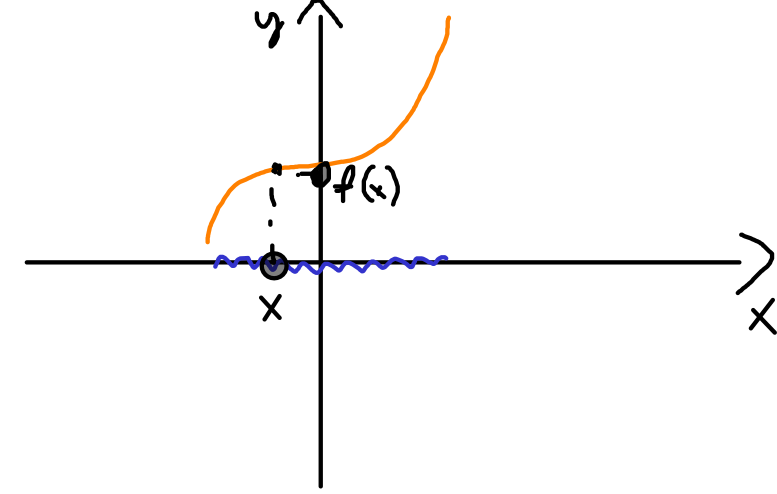
\includegraphics[width=\linewidth]{dim_iniettivita.png}
  	\caption{Dimostrazione Iniettività}
        \label{fig:dim_iniettivita}
\end{figure}


\end{definition}


dove $ f(x) $ è la distanza (con segno) del punto sul grafico dall'asse dell'ascisse



\subsection{Surriettività}\label{sec:surriettività}
\begin{definition}
        $ f: A \to \mathbb{R} $ è surriettiva se $ \forall y \in \mathbb{R} \exists $ 
\end{definition}

\begin{definition}
graficamente possiamo dire che $f : A \to \mathbb{R}$ è surriettiva se $ \forall y_0 \in \mathbb{R} $ la retta $ \{y = y_0\} $ interseca il grafico di $ f $ in almeno un punto.
\end{definition}

\begin{figure}[H]
  	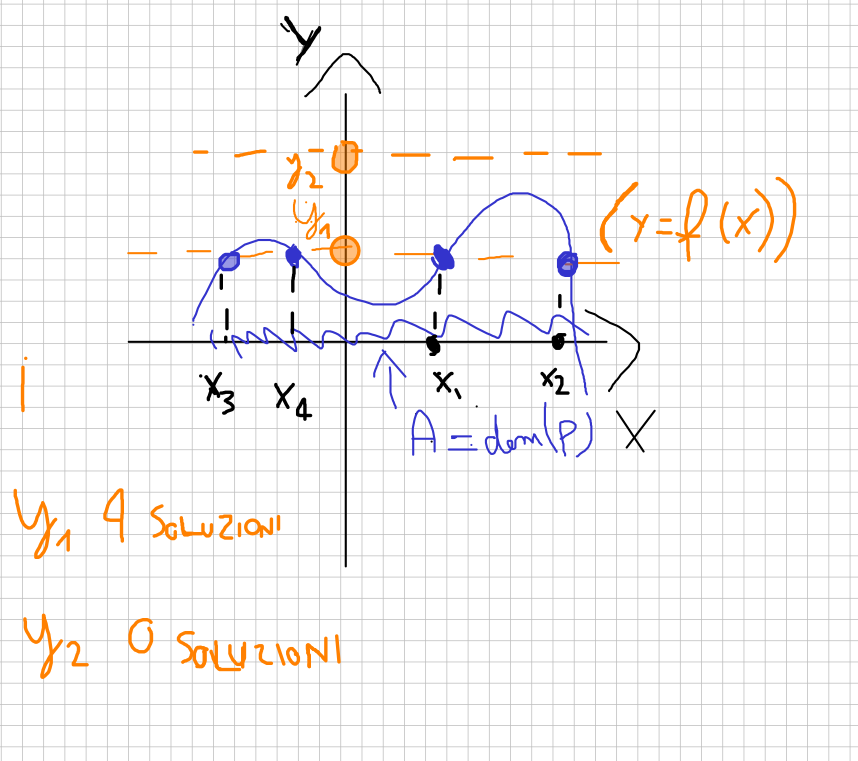
\includegraphics[width=\linewidth]{dim_surriettivita.png}
  	\caption{Dimostrazione grafica surriettività}
        \label{fig:dim_surriettivita}
\end{figure}



\subsection{Biiettiva}\label{sec:biiettiva}
$ f : A \to \mathbb{R} $ è biiettiva se:
\begin{itemize}
        \item $ \forall y_0 \in \mathbb{R} $ la retta $ \{y = y_0\} $ interseca il grafico di $ f $ in almeno un punto.
        \item ogni retta orizzontale intersca il grafico di $ f $ in un punto. 
        \item $ \forall y \in \mathbb{R} \quad f(x) = y$ ha al più una soluzione
\end{itemize}




\newpage
\subsection{Operazioni tra funzioni}\label{sec:operazioni_tra_funzioni}
date $ f,g : A \to \mathbb{R} $ (posso avere anche domini diversi ma allora la funzione che risulterà alla fine avrà come dominio l'intersezione di $ dom(f) $ e $ dom(g) $).

\begin{itemize}
        \item $(f + y)(x) = f(x) + g(x)$
        \item $(f - y)(x) = f(x) - g(x)$
        \item $(f * y)(x) = f(x) * g(x)$
        \item $\Bigg(\dfrac{f}{g}\Bigg)(x) = \dfrac{f(x)}{g(x)}$
        \item $(\lambda f)(x) = \lambda * f(x)$
        \item $ f \circ g (x) = f(g(x))$
\end{itemize}

\begin{tcolorbox}
Possiamo immaginare le funzioni come una black box nella quale inseriamo una valore ed essa ci restituisce un altro valore in base a quello che accade all'intero della black box.
\end{tcolorbox}


Il dominio di $ f \circ g $ è quel numero che:
\todo{Aggiungere il dominio della funzione composta LEZ:4/3}

\begin{exmp}
        Mostriamo alcuni esempi di funzioni composte:
        \begin{align*}
                & e^{x^2} = (f \circ g)(x) \\
                & g(x) = x^2 \quad f(y) = e^y \\
                & f(y(x)) = f(x^2) = e^{x^2}
        \end{align*}
\end{exmp}



\newpage
\subsection{Funzioni inverse}\label{sec:funzione_inversa}
Se $ f : A \to \mathbb{R} $ è iniettiva possiamo costruire la funzione inversa, vedi figura~\ref{fig:dim_iniettivita}. \par
Data $ y \in Im(f) $ posso definire $ x = g(y) $ come l'unica soluzione di $ y = f(x) $
\begin{align*}
        dom(f^{-1}) = Im(f) \\
        Im(f^{-1}) = dom(f) \\
\end{align*}

Una funzione inversa molto comune è l'operazione di radice.

\begin{exmp}
        se $ f : [0, +\infty) \to \mathbb{R} \quad  f(x) = x^2$
        \begin{figure}[H]
          	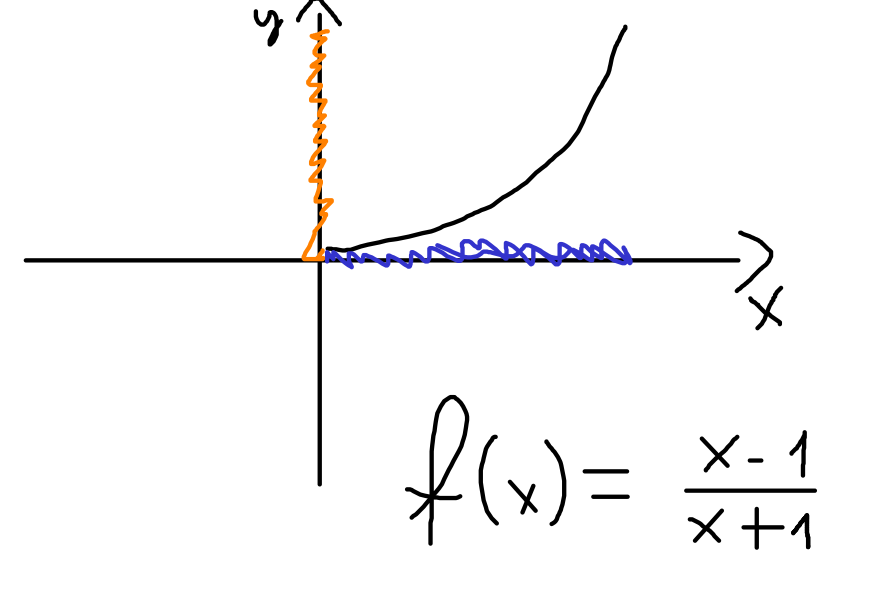
\includegraphics[width=\linewidth]{es_funzione_inversa.png}
          	\caption{}
                \label{fig:es_funzione_inversa}
        \end{figure}

        Vediamo se è iniettiva:
        \begin{equation*}
                \frac{x-1}{x+1} = \frac{y-1}{y+1} 
        \end{equation*}
        \todo{aggiungere dimostrazione LEZ:4/3}
\end{exmp}





























\end{document}
